\chapter{緒言}

\section{研究背景}
油圧アクチュエータは電動アクチュエータと比べ,外力に対する耐衝撃性・質量出力比・最大出力の大きさ・設計の自由度の高さなどに優れており,現在においても使われる分野は多い.
特に建設機械(耐衝撃性や最大出力)や航空機(質量出力比)などの分野では欠かせないものとなっている.
一方で,油漏れを防ぐためのシーリングによる摩擦や,油自身の圧縮性・温度依存性・発火性などの構造や性質に起因する制御性能の低さ,そして電動アクチュエータの高性能化により,現在では制御性能に優れる電動のものが広く使われている.

しかし,電動と油圧を組み合わせた電気油圧式アクチュエータの登場や,計算機能力および制御技術の向上により,特にロボティクスの分野において駆動力として油圧アクチュエータが見直されてきている.
油圧アクチュエータが用いられている例の一つに\figname\ref{fig:PA-2000}に示す6軸油圧マニピュレータPA-2000\cite{IRID}があり,これが本研究において取り扱う対象である.

PA-2000は福島第一原子力発電所の廃炉に向けて燃料デブリを取り出すために,国際原子炉開発機構(IRID)および三菱重工株式会社により開発試作されているマニピュレータである.\cite{河西賢一2018福島第一原子力発電所燃料デブリ横取り出しに向けたロボット開発}.
狭い通路\footnote{CRD交換用開口を通過する.そのため,PA-2000では外形寸法が\SI{700}{mm}$\times$\SI{920}{mm}に抑えられている.}を通過すること,デブリに対する加工反力に耐えることなどの条件を満たすために,質量出力比に優れる油圧アクチュエータが採用されている.
燃料デブリ取り出しは原子炉内という高放射線下で人が立ち入れない環境で行われ,安全に作業を進めるためには,マニピュレータ先端の位置および力を制御する必要がある.
本研究ではこのうち,手先が対象物に接触している状態において発生させる力を制御することに取り組む.

力を制御するにあたり,手先にかかる力を測定してフィードバックを行う必要があるが,力センサなどを用いて直接測定するのではなく,シリンダに取り付けた圧力センサなどを用いて手先の力を推定する手法を開発する.
力センサを用いないことで,マニピュレータ全体の省線化が図れるとともに,複数種類利用することが想定される先端ツールの設計簡略化が期待される.
また,圧力をフィードバックすることにより,マニピュレータ先端が対象物体に触れたときの姿勢に依らず力を推定できることが期待される.

\begin{figure}[t]
    \centering
        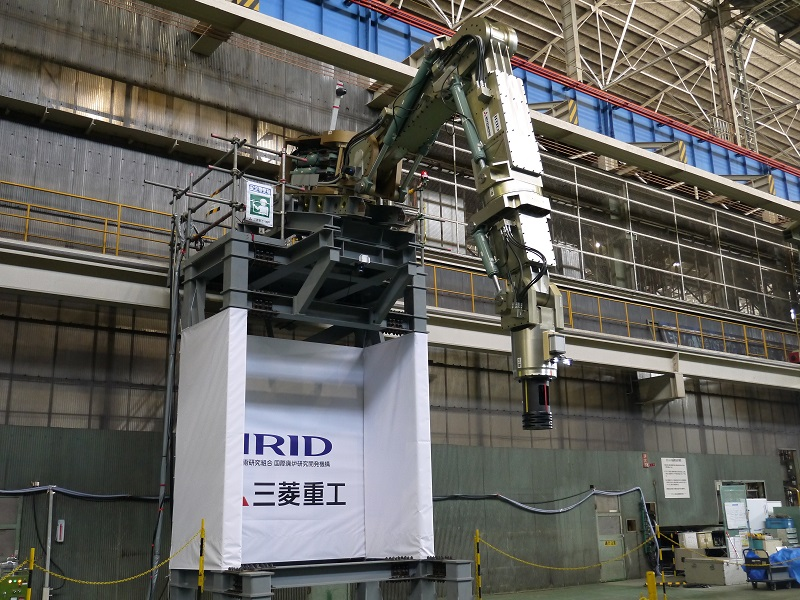
\includegraphics[keepaspectratio, width = .8\linewidth]{contents/緒言/figure/PA-2000.jpg}
        \caption{6-axis Hydraulic Manipulator: PA-2000}
        \label{fig:PA-2000}
\end{figure}

\section{力制御に向けたアプローチ}
力制御に向けたアプローチの概要を\figname\ref{fig:approach_thiswork}に示す.
いきなり6軸油圧マニピュレータで試験を行うのではなく,はじめに油圧シリンダ単体を扱う.
油圧シリンダを対象として力を推定する手法の構築および推定した力を用いたシリンダの力制御を行う.
その後,構築した手法を実験室レベルでORION-7Pへ適用し,最終的にPA-2000への適用を目指す.
ORION-7PはPA-2000と同じ関節配置を持つ油圧マニピュレータである.
本研究では最初の段階である油圧シリンダ単体を対象としてシステム同定を活用した力の推定および力制御を行う.

\begin{figure}[t]
    \centering
        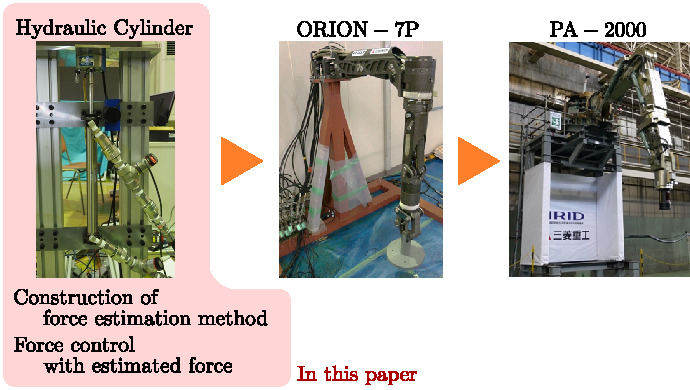
\includegraphics[keepaspectratio, scale=1.0]{contents/緒言/figure/approach_thiswork.pdf}
        \caption{Approach in this work}
        \label{fig:approach_thiswork}
\end{figure}

\section{油圧システムの特徴と関連研究}

\section{本論文の構成}
本論文の構成は次のようになる.
\begin{itemize}
    \item [\ref{sec:FundamentalEquation}章]第一原理に基づいたシステムのモデルの記述をする.これはJelaliらの方法\cite{jelali2012hydraulic}に基づき行う.
    \item [\ref{sec:SystemIdentification}章]油圧システムのシステム同定を行い,力推定の準備をする.
    \item [\ref{sec:ForceControl}章]力制御を行う.
    力制御にあたってはPID制御やI-PD制御,$H_\infty$制御を適用し,比較を行う.
    \item [\ref{sec:IntegrationControl}章] 位置制御と力制御を組み合わせた制御を行う.また,コンプライアンス制御の適用も試みる.
\end{itemize}
